%%%%%%%%%%%%%%%%%%%%%%%%%%%%
% Results
%%%%%%%%%%%%%%%%%%%%%%%%%%%%%
\section{Results}\label{sec:pipeline_experimental_results}

\subsection{Full Pipeline Statistics}\label{sec:full_pipeline_statistics}
We demonstrate the base functionality of \name{} by running our pipeline for all nine priority pathogens using \texttt{gpt-oss-120b}. \name{} completes each report with an average wall clock time of $20$ hours, processing $9,132$ articles at title/abstract screening, $1,102$ at full-text screening and $395$ at data extraction.\footnote{We consider articles processed at each stage based on average across pathogens. See \cref{app:perg_pipeline} for more details.} \Cref{app:report_writeup} explains the report generation process in detail. \Cref{fig:time_comparison} shows the time comparison to human expert estimates, where \name{}'s runtime ($\le$ 1 day) represents a $19.3$-times efficiency gain over the corresponding human processes ($385$ hours).  Since \name{} runs continually, our runtime equates to a 
$58$-times reduction in calendar days (assuming $8$-hour workdays for 
humans). For full-text screening in particular, \name{} is $118$ times faster than humans, reducing a $4$-minute average down to below $2$ seconds per article.  The average cost of running \name{} per SLR varies by model and deployment: for example, self-hosting \texttt{gpt-oss-120b} on two Nvidia H200 GPUs costs approximately USD\$137,\footnote{This cost estimate includes OCR PDF-to-markdown conversion using \texttt{mistral-ocr-2512}.} while using the OpenRouter API reduces the cost to USD\$50 with higher latency as a trade-off. \Cref{app:pipeline_statistics_costs} provides detailed comparisons across models and services.

% Assuming USD\$2.50 per H200 per hour (2 GPUs) plus USD\$36.60 for OCR ($1,102$ articles $\times$ $16.7$ pages at USD\$2 per 1,000 pages via Mistral OCR 3), we estimate a total cost of USD\$137.00 per report for \texttt{gpt-oss-120b}. Costs for ablation models via both H200 and OpenRouter API are provided in Appendix~\ref{app:pipeline_statistics}.}

%, includes \myred{$X$}, and extracts \myred{$X$} data points. This process produces nine novel reports on the evidence base for each pathogen, which we provide in \myred{Appendix X}. \Cref{app:pipeline_statistics} presents further runtime statistics broken down by pathogen and pipeline stage.

%%%%%%%%%%%%%%%%%%%%%%%%%%%%%%%%%%%%%%%%%%%%%%%
% Results — Evaluation Against Ground-truth
%%%%%%%%%%%%%%%%%%%%%%%%%%%%%%%%%%%%%%%%%%%

\subsection{Evaluation Against Ground-truth}\label{sec:PERG_data_evaluation}



\begin{figure*}[t!]
    \centering
    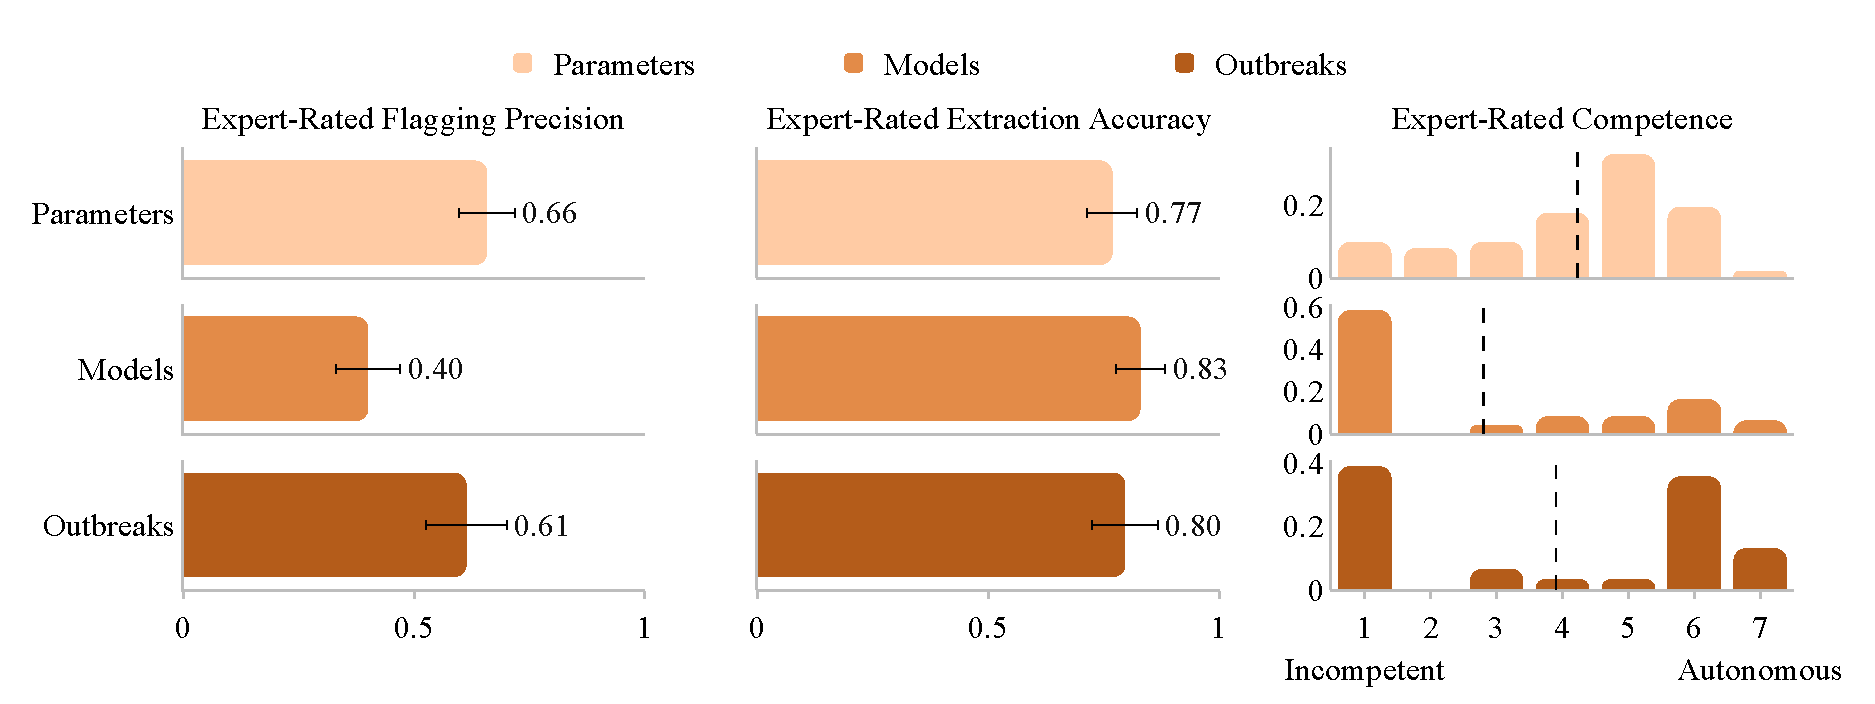
\includegraphics[width=\linewidth]{figures/results/expert_survey.pdf}
    \caption{\textbf{Human expert evaluation of data extraction quality across stages.} We report expert-rated flagging precision, field-level extraction accuracy, and perceived \name{} (\texttt{gpt-oss-120b}) competence for parameter, model, and outbreak extractions, aggregated across six epidemiologists. Error bars denote standard errors, and dashed lines indicate mean competence ratings ($4.2$ for parameters, $2.8$ for models, and $3.9$ for outbreaks).}
    \label{fig:expert_validation_results}
\end{figure*}

%%




\begin{figure*}[t]
    \centering
    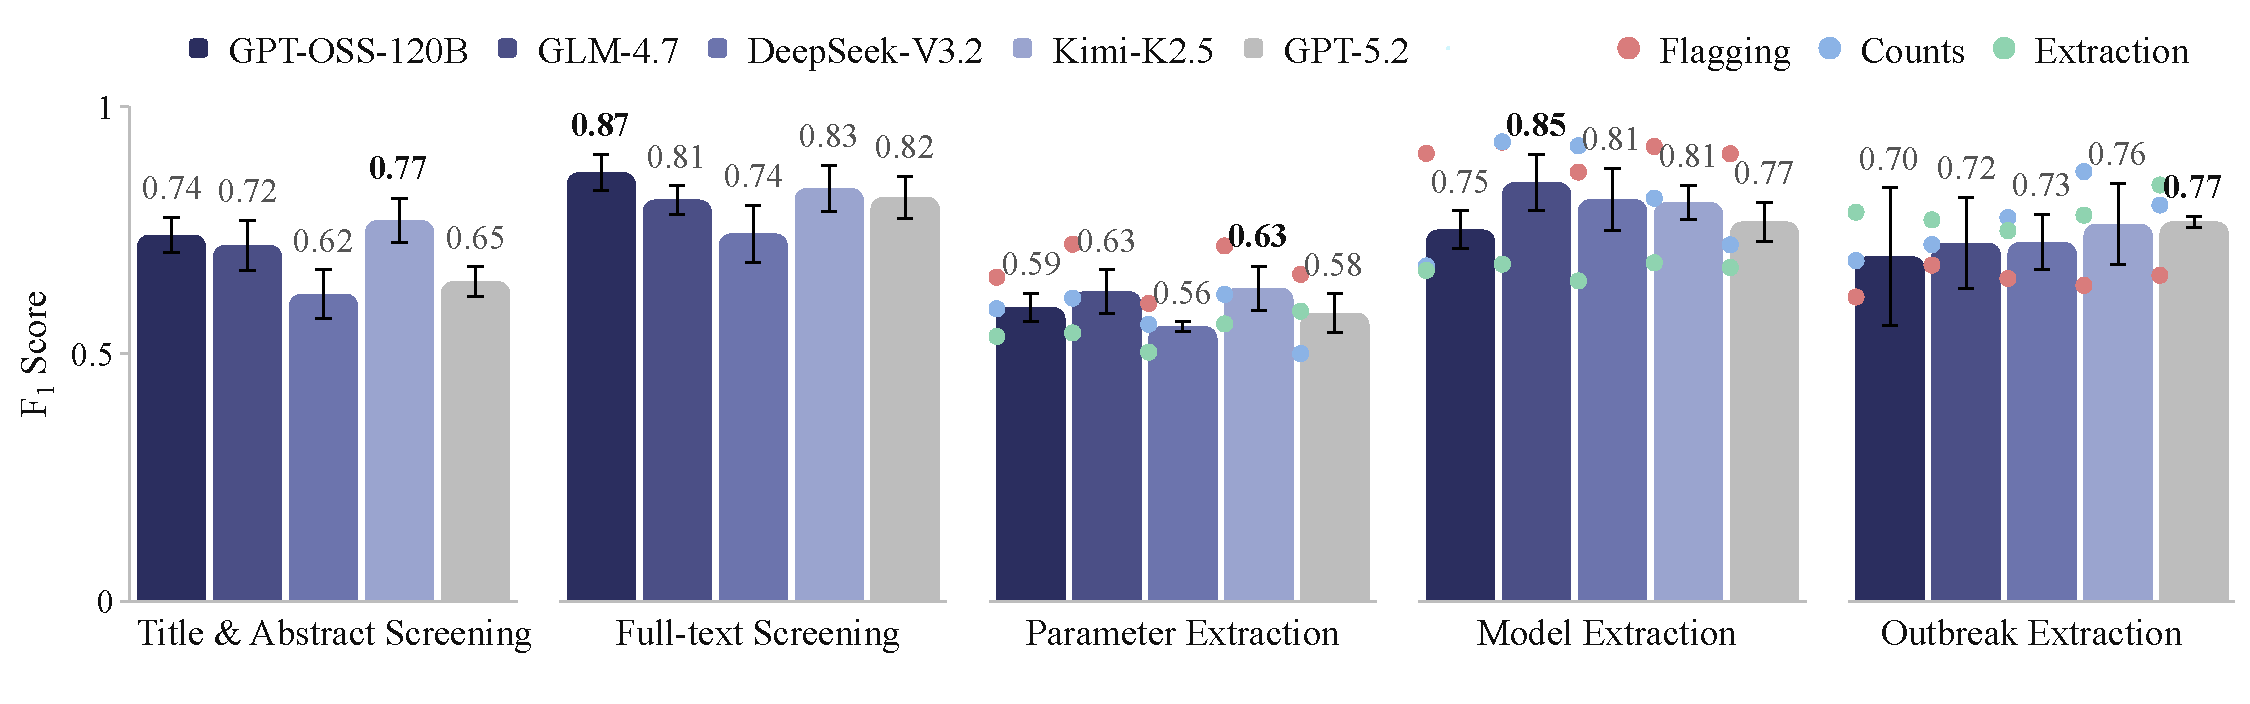
\includegraphics[width=\textwidth]{figures/ablation/model_ablations.pdf}
    \caption{\textbf{Model ablation results with \name{} across all pipeline stages.} Macro F1 is reported for five client models, evaluated separately for each pathogen. Averages are computed over the pathogens evaluated at each stage, following ground-truth availability described in Section~\ref{sec:methods_data}. Error bars indicate one standard deviation across pathogens. For the three data extraction panels, coloured dots show the macro F1 of the Flagging \deflagging{}, Counts \decounts{}, and Extraction \deextraction{} sub-tasks, plotted to the left of each bar. No single model dominates across all stages: \texttt{Kimi-K2.5} and \texttt{gpt-oss-120b} lead screening, while extraction leaders vary by data type. Full pathogen-wise metrics are provided in Appendix~\ref{app:model_ablations}.}
    \label{fig:model_ablation}
\end{figure*}


%%%%%%%%%%%%%%%%%%%%%%%%%%%%%%%%%%%%%%%%%%%%%%%%%%%%
% Evaluation Against Ground-truth — Article Screening
%%%%%%%%%%%%%%%%%%%%%%%%%%%%%%%%%%%%%%%%%%%%%%%%%%%%
\paragraph{Article screening.}
\Cref{fig:fulltext_recall_barchart} compares three article screening strategies tested across the seven evaluated pathogens. Under the default two-stage screening pipeline, \name{} achieves a recall of $0.81$ against ground-truth screening decisions. To contextualise this performance, we consider two ablations. First, we condition full-text screening on ground-truth (human) abstract screening decisions, which improves recall to $0.92$. Second, we omit abstract screening and process all full-texts directly, which improves recall to $0.89$. Both trends are consistent across pathogens (\Cref{fig:fulltext_recall_barchart}). Direct full-text screening thus improves recall over the two-stage pipeline without human involvement, though at a $2.3\times$ increase in screening runtime ($9.55$ vs $4.16$ hours) and a corresponding rise in OCR costs (USD\$36.6 vs USD\$303.2).

\paragraph{Data extraction.}
\Cref{tab:data_extraction_metrics} presents our evaluation results for parameter, model and outbreak extraction. We report average classification measures (precision, recall and $F_1$) for each of our Flagging, Count and Extraction metrics. Across all data types, flagging achieves the highest average $F_1$ ($0.75$), with performance declining progressively through counting ($0.65$) and extraction ($0.63$), reflecting the compounding difficulty of each successive pipeline stage.
See \Cref{app:data_extraction_extended} for complete disaggregated results across all data subtypes, pathogens and individual fields.

%\paragraph{Parameter Extraction} 
\name{} displays high recall ($0.92$) but moderate precision ($0.51$) for parameter class flagging. For parameter extraction counts, this trend reverses, suggesting that the agent identifies many parameter classes as potentially relevant, yet exercises more discretion when producing structured extractions. At the field level, performance is moderate across all pathogens. \name{} achieves near-perfect accuracy for method extraction and for specific uncertainty fields (notably single-type uncertainty), while value fields and population context prove considerably more challenging (See \cref{tab:parameters_detailed_metrics}). 

%\paragraph{Model Extraction} 
\name's model extraction achieves strong flagging performance, with high recall ($0.91$) and precision ($0.90$). This high recall carries through to model counts ($0.99$), indicating that nearly all models from the ground truth data are recovered, albeit with lower precision for counting ($0.52$). At the field level, model extraction attains a precision of $0.63$ and recall of $0.74$: core structural characteristics (model type, stochastic vs.\ deterministic and code availability) are extracted reliably, while complex multi-value fields such as assumptions, interventions and transmission routes remain more challenging (See \cref{tab:models_detailed_metrics} for the complete results).



\begin{table}[b!]
\centering
\caption{\textbf{Evaluation metrics for data extraction stage (averaged across pathogens with $\pm$ deviation).} Results for \name{} (\texttt{gpt-oss-120b}) are reported separately for \textit{Flagging}, \textit{Count}, and \textit{Extraction}, measuring presence identification, quantity accuracy, and value accuracy, respectively. Flagging achieves the strongest performance ($F_1 = 0.75$), followed by counting and extraction. For disaggregated metrics, see \Cref{app:data_extraction_extended}.}
\label{tab:data_extraction_metrics}
\footnotesize
\setlength{\tabcolsep}{3.5pt}
\renewcommand{\arraystretch}{0.97}
\begin{tabular}{lccc}
\toprule
\textbf{Data Type} & \textbf{Precision} & \textbf{Recall} & \textbf{$F_1$ Score} \\
\midrule
\multicolumn{4}{l}{\textbf{Parameters}} \\
\quad \deflagging{} Flagging   & 0.51 ($\pm$ 0.07) & 0.92 ($\pm$ 0.06) & 0.66 ($\pm$ 0.06) \\
\quad \decounts{} Count      & 0.83 ($\pm$ 0.10) & 0.47 ($\pm$ 0.09) & 0.59 ($\pm$ 0.07) \\
\quad \deextraction{} Extraction & 0.52 ($\pm$ 0.03) & 0.57 ($\pm$ 0.04) & 0.54 ($\pm$ 0.02) \\

\midrule

\multicolumn{4}{l}{\textbf{Models}} \\
\quad \deflagging{} Flagging   & 0.90 ($\pm$ 0.04) & 0.91 ($\pm$ 0.05) & 0.91 ($\pm$ 0.04) \\
\quad \decounts{} Count      & 0.52 ($\pm$ 0.05) & 0.99 ($\pm$ 0.01) & 0.68 ($\pm$ 0.04) \\
\quad \deextraction{} Extraction & 0.63 ($\pm$ 0.04) & 0.74 ($\pm$ 0.02) & 0.67 ($\pm$ 0.03) \\

\midrule

\multicolumn{4}{l}{\textbf{Outbreaks}} \\
\quad \deflagging{} Flagging   & 0.63 ($\pm$ 0.06) & 0.76 ($\pm$ 0.05) & 0.61 ($\pm$ 0.09) \\
\quad \decounts{} Count      & 0.66 ($\pm$ 0.17) & 0.72 ($\pm$ 0.28) & 0.69 ($\pm$ 0.22) \\
\quad \deextraction{} Extraction & 0.85 ($\pm$ 0.00) & 0.76 ($\pm$ 0.02) & 0.79 ($\pm$ 0.01) \\

\midrule

\multicolumn{4}{l}{\textbf{Average (across data types)}} \\
\quad \deflagging{} Flagging   & 0.70 ($\pm$ 0.05) & 0.88 ($\pm$ 0.04) & 0.75 ($\pm$ 0.06) \\
\quad \decounts{} Count      & 0.67 ($\pm$ 0.09) & 0.73 ($\pm$ 0.06) & 0.65 ($\pm$ 0.06) \\
\quad \deextraction{} Extraction & 0.62 ($\pm$ 0.07) & 0.67 ($\pm$ 0.03) & 0.63 ($\pm$ 0.05) \\

\bottomrule
\end{tabular}
\end{table}


%\paragraph{Outbreak Extraction} 
We evaluate outbreak extraction only for Lassa and Zika due to a lack of human annotation for Ebola and SARS. Article flagging shows moderate performance across both pathogens (precision $0.63$, recall $0.76$), and outbreak counting shows high variance ($\pm 0.28$ for recall) driven by pathogen-level differences. Despite this, field-level extraction is robust: outbreak extraction achieves the highest precision ($0.85$) amongst all data types, with particular strength in temporal features and case burden (See \cref{tab:outbreak_detailed_metrics}).

%%%%%%%%%$%%%%%$%%%%%%%%%$%%%%%%%%%$%%%%%%%%%$%%%%%%%%%$
% OLD Formatting — Data Extraction Table (ICML Submission
%%%%%%%%%%%%%%%$%%%%%%%%%$%%%%%%%%%$%%%%%%%%%$%%%%%%%%%$


%%%%%%%%%%%%% Table with new (corrected) Param extraction values %%%%%%%%%%%%
% \begin{table*}[t]
%     \centering
%     \caption{\textbf{Evaluation metrics for data extraction stage of \name{} pipeline (with \texttt{gpt-oss-120b}).} \textit{Flagging} validates how well the model identifies the presence of individual data components (epidemiological parameters, transmission models and concluded outbreaks) in each article. \textit{Count} validates the accuracy of extracted quantities, ensuring whether the model correctly identifies the number of data components per article. \textit{Extraction} validates the accuracy of specific values extracted from articles, grouped along data component lines.}
%     \label{tab:data_extraction_metrics}
%     \begin{footnotesize}
%     \begin{tabular}{ll|ccc|ccc|ccc}
%         \toprule
%         \bf \multirow{2}{*}{Data type} & \bf \multirow{2}{*}{Pathogen} & \multicolumn{3}{c|}{\textbf{Flagging}} & \multicolumn{3}{c|}{\textbf{Count}} & \multicolumn{3}{c}{\textbf{Extraction}} \\
%          & & $P$ & $R$ & $F_1$ & $P$ & $R$ & $F_1$ & $P$ & $R$ & $F_1$ \\
%          \midrule
%          \multirow{5}{*}{Parameters} & Lassa & 0.557 & 0.982 & 0.711 & 1.000 & 0.346 & 0.514 & 0.578 & 0.535 & 0.551 \\
%         & Ebola & 0.596 & 0.917 & 0.722 & 0.794 & 0.470 & 0.590 & 0.485 & 0.539 & 0.501 \\
%         & SARS & 0.500 & 0.815 & 0.620 & 0.804 & 0.610 & 0.694 & 0.514 & 0.633 & 0.558 \\
%         & Zika & 0.403 & 0.957 & 0.567 & 0.720 & 0.468 & 0.567 & 0.515 & 0.574 & 0.531 \\
%          \cmidrule{2-11}
%          & Average & 0.514 & 0.918 & \multicolumn{1}{c|}{0.655} &  0.829 & 0.473 & \multicolumn{1}{c|}{0.591} & 0.523 & 0.570 & 0.535 \\
%          \midrule
%          \multirow{5}{*}{Models} & Lassa & 0.909 & 1.000 & 0.952 & 0.600 & 1.000 & 0.750 & 0.687 & 0.699 & 0.690 \\
%          & Ebola & 0.876 & 0.952 & 0.912 & 0.500 & 1.000 & 0.667 & 0.606 & 0.680 & 0.636 \\
%          & SARS & 0.841 & 0.841 & 0.841 & 0.486 & 0.971 & 0.648 & 0.610 & 0.683 & 0.638 \\
%          & Zika & 0.785 & 0.911 & 0.843 & 0.483 & 0.977 & 0.646 & 0.683 & 0.753 & 0.706 \\
%          \cmidrule{2-11}
%          & Average & 0.853 & 0.926 & 0.887 & 0.517 & 0.987 & 0.678 & 0.647 & 0.704 & 0.668 \\
%          \midrule
%          \multirow{3}{*}{Outbreaks} & Lassa & 0.690 & 0.816 & 0.705 & 0.833 & 1.000 & 0.909 & 0.864 & 0.740 & 0.778 \\
%          & Zika & 0.576 & 0.713 & 0.525 & 0.489 & 0.449 & 0.468 & 0.870 & 0.780 & 0.812 \\
%          \cmidrule{2-11}
%          & Average & 0.633 & 0.765 & 0.615 & 0.661 & 0.724 & 0.689 & 0.867 & 0.760 & 0.795 \\
%           \midrule
%           \bf Average & & 0.644 & 0.905 & 0.718 & 0.649 & 0.757 & 0.664 & 0.720 & 0.723 & 0.710 \\
%           \bottomrule
%     \end{tabular}
%     \end{footnotesize}
% \end{table*}


%%%%%%%%%%%%% Table with original (official ICML submission) Param extraction values %%%%%%%%%%%%

% \newcolumntype{C}{>{\centering\arraybackslash}X}




% \begin{table*}[t]
% \footnotesize
%     \centering
%     \caption{\textbf{Evaluation metrics for data extraction stage of \name{} pipeline.} \textit{Flagging} validates how well the model identifies the presence of individual data components (epidemiological parameters, transmission models and concluded outbreaks) in each article. \textit{Count} validates the accuracy of extracted quantities, ensuring whether the model correctly identifies the number of data components per article. \textit{Extraction} validates the accuracy of specific values extracted from articles, grouped along data component lines.\SP{Add Table is specific to gpt-oss-120b}}
%     \label{tab:data_extraction_metrics}
%     %\scriptsize
%     \begin{tabularx}{0.95\textwidth}{ll|CCC|CCC|CCC}
%         \toprule
%         \bf \multirow{2}{*}{Data type} & \bf \multirow{2}{*}{Pathogen} & \multicolumn{3}{c|}{\textbf{Flagging}} & \multicolumn{3}{c|}{\textbf{Count}} & \multicolumn{3}{c}{\textbf{Extraction}} \\
%          & & $P$ & $R$ & $F_1$ & $P$ & $R$ & $F_1$ & $P$ & $R$ & $F_1$ \\
%          \midrule
%          \multirow{5}{*}{Parameters} & Lassa & 0.438 & 0.955 & 0.600 & 0.800 & 0.545 & 0.649 & 0.594 & 0.655 & 0.615 \\
%                                      & Ebola & 0.510 & 0.958 & 0.665 & 0.798 & 0.538 & 0.643 & 0.581 & 0.604 & 0.583 \\
%                                      & SARS  & 0.463 & 0.954 & 0.623 & 0.909 & 0.667 & 0.769 & 0.548 & 0.655 & 0.573 \\
%                                      & Zika  & 0.352 & 0.949 & 0.514 & 0.596 & 0.418 & 0.491 & 0.519 & 0.581 & 0.541 \\
%          \cmidrule{2-11}
%          & Average & 0.441 & 0.954 & \multicolumn{1}{c|}{0.601} & 0.776 & 0.542 & \multicolumn{1}{c|}{0.638} & 0.561 & 0.624 & 0.578 \\
%          \midrule
%          \multirow{5}{*}{Models} & Lassa & 0.909 & 1.000 & 0.952 & 0.600 & 1.000 & 0.750 & 0.687 & 0.699 & 0.690 \\
%          & Ebola & 0.876 & 0.952 & 0.912 & 0.500 & 1.000 & 0.667 & 0.606 & 0.680 & 0.636 \\
%          & SARS & 0.841 & 0.841 & 0.841 & 0.486 & 0.971 & 0.648 & 0.610 & 0.683 & 0.638 \\
%          & Zika & 0.785 & 0.911 & 0.843 & 0.483 & 0.977 & 0.646 & 0.683 & 0.753 & 0.706 \\
%          \cmidrule{2-11}
%          & Average & 0.853 & 0.926 & 0.887 & 0.517 & 0.987 & 0.678 & 0.647 & 0.704 & 0.668 \\
%          \midrule
%          \multirow{3}{*}{Outbreaks} & Lassa & 0.690 & 0.816 & 0.705 & 0.833 & 1.000 & 0.909 & 0.864 & 0.740 & 0.778 \\
%          & Zika & 0.576 & 0.713 & 0.525 & 0.489 & 0.449 & 0.468 & 0.870 & 0.780 & 0.812 \\
%          \cmidrule{2-11}
%          & Average & 0.633 & 0.765 & 0.615 & 0.661 & 0.724 & 0.689 & 0.867 & 0.760 & 0.795 \\
%           \midrule
%           \bf Average & & 0.644 & 0.905 & 0.718 & 0.649 & 0.757 & 0.664 & 0.720 & 0.723 & 0.710 \\
%           \bottomrule
%     \end{tabularx}
% \end{table*}